\section*{Model description}
The work will be based on the latest release series of the \gls{cesm} and its components, \gls{clm}~5 including \gls{bvoc} emissions (\gls{megan} model \parencite{ACP:Guenther2006}, \gls{cam}~6 with online (super-fast) chemistry (\gls{impact} model, \textcite{JGR:Rotman2004}). 
In the following, I will give a brief account of the most relevant parts of the aforementioned model components of \gls{cesm}, \gls{clm} including \gls{megan}, and \gls{cam}. After that I first present the Lombardozzi model of ozone damage and then elaborate on my more process oriented, new plant physiological model of ozone damage and its integration into \gls{clm}.

In \gls{clm}~5, \textbf{photosynthesis} (and hence the carbon cycle) is tied to \textbf{plant nutrient dynamics} (dark gray cycles depicted in Fig.~\ref{fig:ozone_odina}) which incorporates the \textbf{\gls{fun}} model \parencites{GBC:Fisher2010}{JGR:Brzostek2014}{GCB:Shi2015}. The concept of \gls{fun} is that nitrogen uptake requires an investment of energy (e.g. carbon) and that there is a large number of potential sources of nitrogen available in the environment. The ratio of carbon invested to acquire nitrogen is therefore treated as a cost. \gls{fun} calculates the rate of symbiotic nitrogen fixation for nitrogen passed directly to the plant and passed as inorganic ammonium to the soil \parencite{GBC:Cleveland1999}, separately. Nutrient limitation is represented by a variable plant \ch{C:N} ratio which allows plants to adjust their \ch{C:N} ratio at the leaf level at the cost of nitrogen \parencite{JAMES:Ghimire2016}. The \textbf{\gls{luna}} model \parencites{STE:Xu2019}{GMD:Ali2016} finally links these with photosynthesis. The \gls{luna} model calculates photosynthetic capacity based on optimization of the use of leaf nitrogen under different environmental conditions. \textbf{Stomatal conductance} is based on this \textbf{nitrogen-limited photosynthesis} rather than on potential photosynthesis. The maximum stomatal conductance is obtained from the \textbf{Medlyn stomatal conductance} model \parencite{GCB:Medlyn2011} which is preferred over Ball-Berry-type models \parencite{BallBerry1987} for it’s more realistic behavior at low humidity levels (high vapor pressure deficit) \parencites{PR:Rogers2013}{NP:Rogers2017}.  
As a \textbf{plant hydraulic stress} routine explicitly models water transport through the vegetation according to a simple hydraulic framework \parencite{JAMES:Kennedy2019}, stomatal conductance is also a function of prognostic leaf water potential and hence forced by transpiration. Water stress is calculated as the ratio of attenuated stomatal conductance to maximum stomatal conductance.

\textbf{Biogenic emissions} from vegetation are not integrated into the framework described above but handled by \gls{megan} \textcite{ACP:Guenther2006}. \gls{megan} takes above canopy atmospheric forcing, e.g. solar radiation, temperature, and moisture, and \ch{[CO_2]} as input variables. It only depends on vegetation through \gls{lai} which can be either prescribed (\gls{sp} mode) or dynamic (\gls{bgc} mode) and \gls{pft}. In \gls{clm}~5, \gls{megan} version 2.1 \parencite{GMD:Guenther2012} is implemented. \gls{megan}~2.1 includes 147 chemical compounds which can be subset and grouped together (e.g. \emph{isoprene} = pentane + hexane + heptane + tricyclene). In \gls{clm}, trapping of emissions inside of the canopy is explicitly disabled (escape efficiency set to 1).

In \textbf{\gls{cam}-chem}, \textbf{dry deposition} follows the resistance approach originally described by \textcites{AE:Wesely1989}{AE:Walcek1986} and updated sequentially \parencites{AE:Walmsley1996}{AE:Wesely2000}. All deposited chemical species are mapped to a weighted-combination of ozone and sulfur dioxide depositions to characterize their oxidation potential versus solubility in water. Solubility is dependent on the effective Henry’s law coefficient of the species. All species in the mechanism are per default affected by dry deposition if deposition velocities are defined. 
The computation of \textbf{deposition velocities} (or resistances) ties \gls{cam}-chem to \gls{clm}. Dry deposition velocities vary with \gls{pft}. A grid-averaged velocity is computed as the weighted-mean over all land cover types. The impact from changes in land cover, land use or climate are thus reflected \parencite{GMD:Lamarque2012}. 

\begin{wrapfigure}[]{L}[0pt]{0.5\textwidth}
  % R - floating; r - h! [narrow lines] <- reduce whitespace below [17]
  \centering
  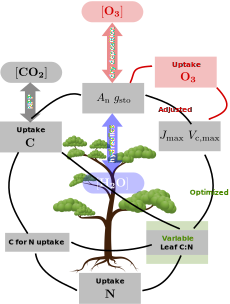
\includegraphics[width=0.48\textwidth]{ozone_luna_scheme}
  \caption{Schematic view of existing process modeling in \gls{clm}~5 and \gls{odina} model in red. Round boxes represent effects on and coupling to atmospheric components of the model (\gls{cam}-chem), e.g. a change in atmospheric concentration of carbon dioxide \ch{[CO_2]}, ozone \ch{[O_3]}, and water vapor \ch{[H_2O]}. Squared boxes represent processes in the land model (\gls{clm}). Plants invest carbon to take up nutrients. A variable carbon to nitrogen ratio (\ch{C:N}) at leaf level determines the optimized electron transport ($\mathrm{J_{max}}$) and carboxylation rate ($\mathrm{V_{cmax}}$). Photosynthesis ($\mathrm{A_n}$) and stomatal conductance ($\mathrm{g_{sto}}$) are dependent on these as well as on plant hydraulics for water transport (blue). Ozone reduces $\mathrm{J_{max}}$ and $\mathrm{V_{cmax}}$ and hence interferes with the whole cycle.
}
  \label{fig:ozone_odina}
\end{wrapfigure}

At present, \textbf{ozone damage} on vegetation is not accounted for by default in \gls{cesm}. There are two reasons for this: 
\begin{enumerate}
  \itemsep0em
\item Ozone fluxes from \gls{cam}-chem are not coupled to \gls{clm} 
\item Running \gls{clm} as stand-alone would necessarily need surface ozone fields which are highly uncertain in available global products (Falk et al. 2021 in preparation).
\end{enumerate}
Ozone damage in \gls{clm}~5 is based on the work of Lombardozzi \parencite{Oe:Lombardozzi2012} which showed an effective decoupling of An and gsto under high \gls{cuo}, with gsto being less sensitive to cumulative uptake of ozone. If taken into consideration this will improve global predictions of GPP and transpiration considerably \parencite{BGS:Lombardozzi2012}, especially in the tropics as also shown by \textcite{ACP:Pacifico2015} and \textcite{ACP:Pacifico2015}. In this implementation, damage coefficients for gsto and An are defined for coniferous, deciduous, and non-woody \glspl{pft}, respectively. \gls{cuo} can be regulated through an uptake threshold $\Phi_\mathrm{th}$. A healing factor is computed based on change in \gls{lai} (growth of new leaves).

The \textbf{\gls{odina}} model, I deduce a linear relationship between an average cumulative uptake of ozone (\gls{cuo}) and $\mathrm{J_{max}}$ relative to a control experiment from a limited number of peer reviewed research articles published in recent years. I take advantage of already existing, scientifically validated modules in \gls{clm} (e.g. \gls{fun}, \gls{luna}). The integration of \gls{odina} into the existing framework of \gls{clm}5 is schematically depicted in Fig. 2. \gls{odina} also builds on previous efforts by \textcites{BGS:Lombardozzi2012}{Oe:Lombardozzi2012}. A comprehensive database of experimental data for implementation of an ozone damage module \parencite{BGS:Lombardozzi2013} will be used for model evaluation of \gls{odina}. The \gls{odina} model can be used to study ozone effects on the \ch{C:N} ratio. The purpose of this project is to establish the coupling of \gls{clm}~5 to \gls{cam}-chem with respect to ozone through dry deposition and evaluate the comprehensive two-way coupling of ozone-vegetation in the light of climate change.
